\chapter{Experiments}
\label{chap:experiments}

This chapter evaluates whether RapidGS reduces training cost while remaining
within the quality range of standard 3D Gaussian Splatting (3DGS). The
experiments are
organized around the thesis contributions rather than individual code changes:
end-to-end acceleration, structure control, compact rasterization, fused
backward/update, and cross-dataset generalization.

\section{Protocol}

The main benchmark contains the nine Mip-NeRF 360 scenes: bicycle, flowers,
garden, stump, treehill, room, counter, kitchen, and bonsai. Additional
generalization experiments use the train and truck scenes from Tanks and
Temples and the drjohnson and playroom scenes from Deep Blending. All methods
use the same COLMAP reconstruction for a scene. PSNR, SSIM, paper-style VGG
LPIPS, training time, wall time, peak allocated VRAM, and final Gaussian count
are recorded. Lower LPIPS and time are better; higher PSNR and SSIM are better.

Unless otherwise stated, RapidGS uses 23,000 iterations, five score views,
compact-box multiplier $m=0.75$, VCD, and late VCP. The
main, ablation, and schedule-sweep tables contain one deterministic run per
scene. Results with a different score-view budget or compact multiplier are
not treated as repeats of the main configuration.

\section{Main Mip-NeRF 360 Result}

\begin{table}[H]
\centering
\caption{Nine-scene mean comparison on Mip-NeRF 360.}
\label{tab:main-result}
\begin{tabular}{lrrrrr}
\toprule
Method & Train time (s) & PSNR & SSIM & LPIPS & Gaussians \\
\midrule
Original 3DGS & 1053.54 & 27.5963 & 0.8153 & 0.2138 & 2.625M \\
FastGS & 235.93 & 27.9330 & 0.8200 & 0.2160 & 1.161M \\
RapidGS & \textbf{152.47} & \textbf{28.1586} & \textbf{0.8289} &
\textbf{0.2073} & 1.086M \\
\bottomrule
\end{tabular}
\end{table}

RapidGS is $6.91\times$ faster than the original 3DGS baseline and 35.4\%
faster than FastGS. It also improves all three mean image
quality metrics in this comparison. This establishes that the short schedule
does not obtain speed only by accepting a lower reconstruction-quality target.

\begin{figure}[H]
\centering
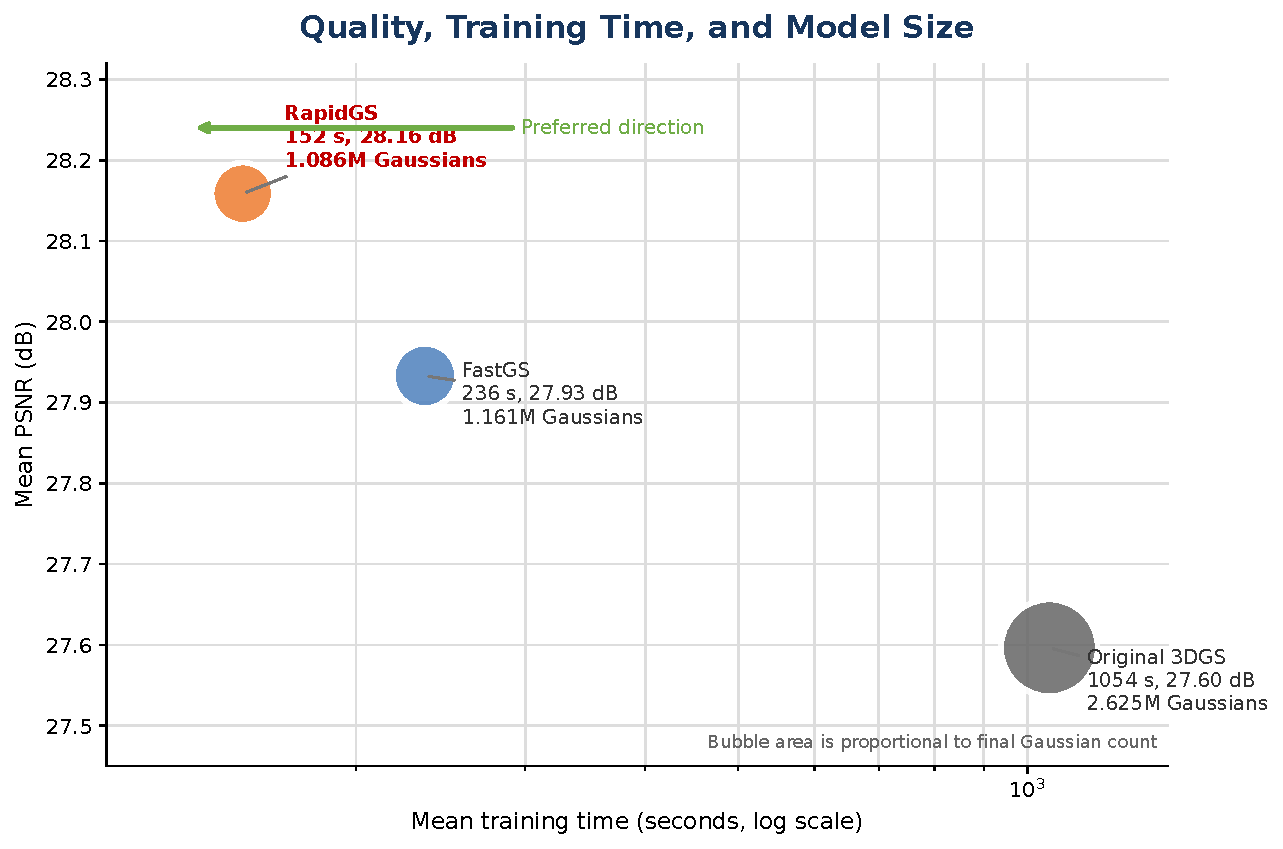
\includegraphics[width=0.88\textwidth]{figures/quality_speed_tradeoff.pdf}
\caption{Joint comparison of mean reconstruction quality, training time, and
final model size on the nine Mip-NeRF 360 scenes. Bubble area is proportional
to the final Gaussian count. RapidGS moves toward the preferred upper-left
region: higher PSNR, shorter training time, and a smaller representation.}
\label{fig:quality-speed-tradeoff}
\end{figure}

\section{Qualitative Comparison}

Figure~\ref{fig:qualitative-all-scenes} compares aligned crops from held-out
views of all nine Mip-NeRF 360 scenes. The renderings are resized to a common
display width because the saved RapidGS main run uses a different output
resolution from the two 30k baselines. No sharpening, denoising, or color
correction is applied. The examples were selected from textured local regions
where RapidGS has lower local image error than both baselines. They therefore
illustrate favorable detail cases rather than an unbiased estimate of average
visual quality; the aggregate metrics in Table~\ref{tab:main-result} provide
the latter comparison.

\begin{figure}[H]
\centering
\includegraphics[width=\textwidth,height=0.79\textheight,keepaspectratio]{figures/qualitative_all_scenes.png}
\caption{Qualitative comparison across all nine Mip-NeRF 360 scenes. The first
column shows the full ground-truth test view; the remaining columns show an
aligned crop from the ground truth, original 3DGS, FastGS, and RapidGS. The
crops emphasize thin structures and high-frequency textures. RapidGS remains
visually competitive with the 30k baselines while using a 23k training
schedule.}
\label{fig:qualitative-all-scenes}
\end{figure}

\section{Structure-Control Ablation}

The structure ablation evaluates complete contribution-level mechanisms rather
than individual implementation changes. ``No VCP'' disables only late
view-consistency pruning.
``No VCD'' retains VCP but removes multi-view consistent densification.
``Gradient only'' removes both VCD and VCP,
leaving the conventional gradient-driven structure rule.

\begin{table}[H]
\centering
\caption{Matched structure-control ablation on all nine Mip-NeRF 360 scenes.}
\label{tab:structure-ablation}
\begin{tabular}{lrrrrr}
\toprule
Configuration & Time (s) & PSNR & SSIM & LPIPS & Gaussians \\
\midrule
Full RapidGS & 152.47 & \textbf{28.1586} & 0.8289 & 0.2073 & 1.086M \\
No VCP & \textbf{147.35} & 28.1261 & 0.8285 & 0.2065 & 1.211M \\
No VCD & 198.85 & 27.9790 & 0.8310 & 0.1970 & 1.816M \\
Gradient only & 205.07 & 28.0574 & \textbf{0.8319} & \textbf{0.1958} & 2.234M \\
\bottomrule
\end{tabular}
\end{table}

\begin{figure}[H]
\centering
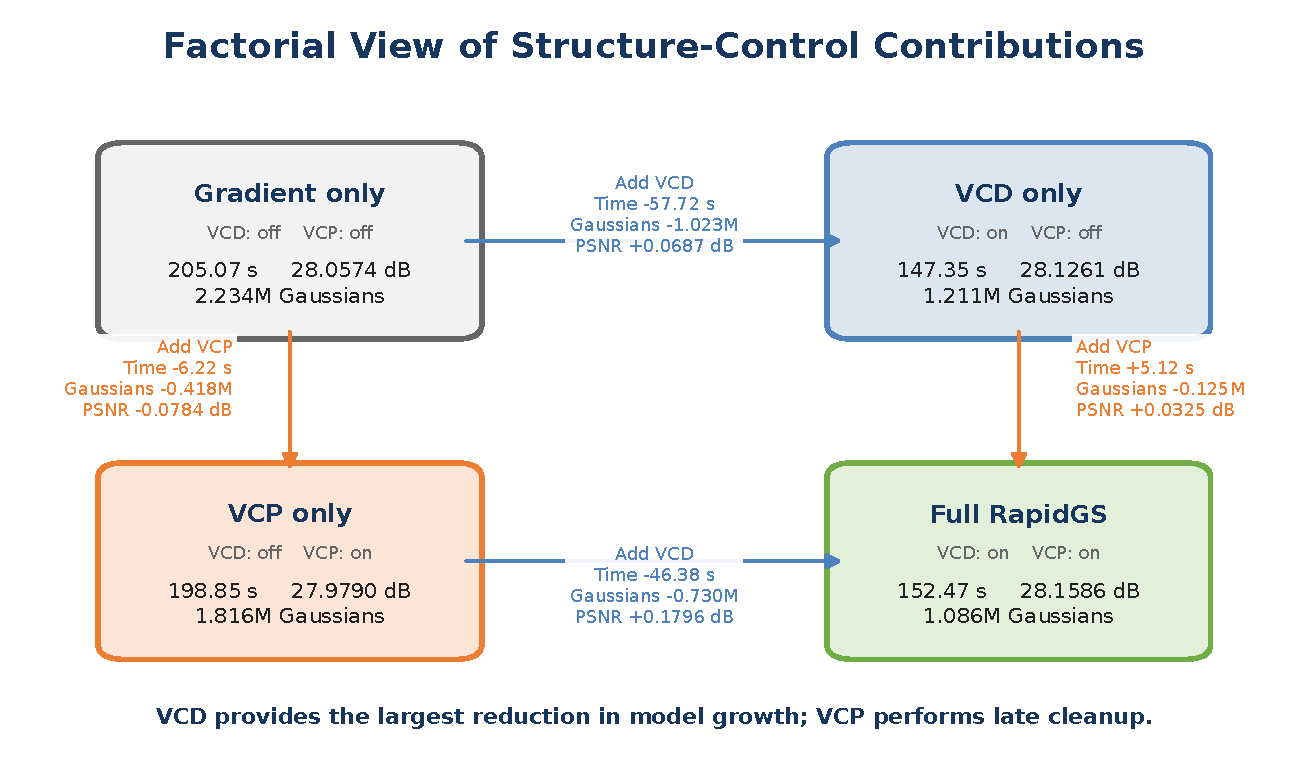
\includegraphics[width=\textwidth]{figures/structure_control_contributions.pdf}
\caption{Factorial view of the two structure-control contributions. Horizontal
arrows add VCD and vertical arrows add VCP. Each arrow
reports the change relative to its source configuration. This layout exposes
the interaction between the mechanisms without implying that the ablations
form a single linear sequence.}
\label{fig:structure-control-contributions}
\end{figure}

VCP is not a standalone speed optimization: its callback costs about 5.1
seconds in the mean result, but it removes approximately 10.3\% of the final
Gaussians and slightly improves PSNR. VCD is the principal
structure-cost control. Removing it increases mean training time by 30.4\% and
the final Gaussian count by 67.2\%. Removing both structure mechanisms
increases time by 34.5\% and more than doubles the final Gaussian count.
The lower LPIPS of the larger ablations is a model-size trade-off rather than a
free improvement, because it requires substantially more training work and
memory.

Three-scene traces on bicycle, garden, and room explain the time increase. At
iteration 23,000, the full method averages 1.514M Gaussians, 1.518M effective
Gaussian--tile instances, and 6.18 ms for the sampled training step. Removing
VCD raises these values to 2.404M, 1.805M, and 8.43 ms. The
gradient-only variant reaches 3.089M, 1.972M, and 9.91 ms. Thus, score-render
overhead is amortized by reducing later rasterization and backward work.

\section{Score Sensitivity}

The score mechanism has two direct budget parameters: the number of sampled
score views $K$ and the densification threshold $\tau_s$. Tables
\ref{tab:score-view-sensitivity} and \ref{tab:score-threshold-sensitivity}
vary one parameter at a time while keeping the 23k schedule, compact multiplier
$0.75$, random seed, and all other settings fixed.

\begin{table}[H]
\centering
\caption{Score-view budget sensitivity on all nine Mip-NeRF 360 scenes.}
\label{tab:score-view-sensitivity}
\begin{tabular}{rrrrrr}
\toprule
$K$ & Time (s) & PSNR & SSIM & LPIPS & Gaussians \\
\midrule
1 & \textbf{124.00} & 27.9743 & 0.8242 & 0.2175 & 0.784M \\
3 & 140.57 & 28.1571 & 0.8286 & 0.2086 & 1.035M \\
5 & 152.47 & \textbf{28.1586} & \textbf{0.8289} & \textbf{0.2073} & 1.086M \\
10 & 149.29 & 28.1329 & 0.8286 & 0.2074 & 1.092M \\
20 & 152.03 & 28.0578 & 0.8271 & 0.2086 & 1.047M \\
\bottomrule
\end{tabular}
\end{table}

One view is insufficient: it is fast and compact, but loses 0.18 dB and
degrades both SSIM and LPIPS relative to $K=5$. Three views recover nearly all
PSNR and SSIM at lower cost, although LPIPS remains 0.0013 worse. Increasing
the budget to 10 or 20 does not consistently improve quality and adds score
rendering work. The main value $K=5$ is therefore a conservative quality
choice, not a uniquely optimal point; $K=3$ is a reasonable faster operating
point when perceptual quality can be relaxed slightly.

\begin{table}[H]
\centering
\caption{Densification score-threshold sensitivity with $K=5$.}
\label{tab:score-threshold-sensitivity}
\begin{tabular}{lrrrrr}
\toprule
$\tau_s$ & Time (s) & PSNR & SSIM & LPIPS & Gaussians \\
\midrule
No gate & 198.85 & 27.9790 & \textbf{0.8310} & \textbf{0.1970} & 1.816M \\
2 & 154.76 & \textbf{28.1611} & 0.8301 & 0.2034 & 1.217M \\
5 & 152.47 & 28.1586 & 0.8289 & 0.2073 & 1.086M \\
8 & \textbf{137.85} & 28.0815 & 0.8260 & 0.2103 & \textbf{0.980M} \\
\bottomrule
\end{tabular}
\end{table}

Lowering the threshold to 2 admits more growth, improving LPIPS and SSIM but
increasing the final model by 12.0\% relative to the main configuration.
Raising it to 8 saves 9.6\% training time and reduces the model by 9.8\%, but
loses 0.077 dB and degrades SSIM and LPIPS. Removing the gate produces the
largest model and the highest training cost. Threshold 5 lies between the
quality-oriented value 2 and the speed-oriented value 8, supporting its use as
the main balanced setting.

\section{Compact Rasterization and Schedule}

\begin{table}[H]
\centering
\caption{Contribution-level compact rasterization ablation over nine scenes.}
\label{tab:compact-on-off}
\begin{tabular}{lrrrrrr}
\toprule
Coverage & Time (s) & PSNR & SSIM & LPIPS & GS & VRAM (GB) \\
\midrule
Compact & \textbf{152.47} & \textbf{28.1586} & \textbf{0.8289} & \textbf{0.2073} & 1.086M & \textbf{5.04} \\
Bounding-box only & 192.06 & 28.0873 & 0.8280 & 0.2084 & \textbf{1.065M} & 5.54 \\
\bottomrule
\end{tabular}
\end{table}

The bounding-box-only control uses the standard conservative three-sigma projected
radius and emits every tile in the resulting rectangle. It changes no
structure-control, loss, or optimizer setting. Compact coverage reduces mean
training time by 20.6\% and peak allocated memory by 0.50 GB while preserving
the same quality region. The small differences in final Gaussian count arise
because changed tile participation also changes the accumulated
densification gradients.

\begin{table}[H]
\centering
\caption{Compact-box multiplier sweep with a common score-view budget of ten.}
\label{tab:compact-ablation}
\begin{tabular}{lrrrr}
\toprule
$m$ & Time (s) & PSNR & SSIM & LPIPS \\
\midrule
0.75 & 155.76 & 28.1058 & 0.8279 & 0.2071 \\
1.00 & \textbf{155.57} & \textbf{28.1261} & \textbf{0.8284} & \textbf{0.2072} \\
1.25 & 166.70 & 28.1058 & 0.8279 & 0.2078 \\
\bottomrule
\end{tabular}
\end{table}

The multiplier sweep is a sensitivity analysis within the enabled compact
path, not an on/off ablation. The values $m=0.75$ and $m=1.0$ are numerically
close in this single-run sweep, while $m=1.25$ adds 7.0\%--7.2\% training time without a
quality gain. The result supports compact tile assignment, but it does not
justify claiming that $0.75$ is universally optimal.

\begin{table}[H]
\centering
\caption{Controlled RapidGS schedule sweep over nine scenes under the main
$m=0.75$, $K=5$ configuration.}
\label{tab:schedule-sweep}
\begin{tabular}{lrrrrr}
\toprule
Iterations & Time (s) & PSNR & SSIM & LPIPS & GS \\
\midrule
21k & \textbf{133.60} & 28.0245 & 0.8270 & 0.2095 & \textbf{1.073M} \\
22k & 139.29 & 28.1163 & 0.8279 & 0.2085 & 1.082M \\
23k & 152.47 & \textbf{28.1586} & 0.8289 & 0.2073 & 1.086M \\
25k & 156.10 & 28.1043 & 0.8284 & 0.2059 & 1.084M \\
27k & 167.41 & 28.1293 & \textbf{0.8297} & \textbf{0.2047} & 1.085M \\
\bottomrule
\end{tabular}
\end{table}

All settings change only the total iteration count, the corresponding
position-learning-rate horizon, and the VCP end boundary. The 21k setting is
12.4\% faster than 23k but loses 0.134 dB PSNR and degrades both SSIM and
LPIPS. The 22k setting narrows this gap, but 23k gives the highest PSNR and a
better balance across all three metrics. Extending the schedule to 25k or 27k
improves LPIPS, but does not improve PSNR; 27k also costs 9.8\% more training
time. These results support 23k as the quality-constrained operating point
rather than the shortest or longest schedule tested.

\begin{table}[H]
\centering
\caption{Matched 23k versus 30k schedule control under the main RapidGS
configuration.}
\label{tab:schedule-ablation}
\begin{tabular}{lrrrrr}
\toprule
Iterations & Time (s) & PSNR & SSIM & LPIPS & GS \\
\midrule
23k & \textbf{152.47} & 28.1586 & \textbf{0.8289} & 0.2073 & 1.086M \\
30k & 183.27 & \textbf{28.1734} & \textbf{0.8289} & \textbf{0.2054} & 1.086M \\
\bottomrule
\end{tabular}
\end{table}

The matched 30k control keeps all structure-edit boundaries and the final
learning-rate tail unchanged, extending only the number of optimization
steps. The extra 7,000 iterations cost 20.2\% more training time for 0.015 dB
mean PSNR and 0.0019 LPIPS. The selected 23k schedule is therefore a
quality-constrained operating point rather than the shortest possible run.

\section{Fused Backend}

The fused CUDA path performs gradient propagation, Adam moment updates, and
parameter updates in one backend operation. A reduced 5,000-Gaussian fixture
checks the fused Adam mutation against the explicit Adam equation; the maximum
absolute parameter error is below $10^{-6}$. Central finite differences also
confirm the gradient directions for all parameter groups, although geometric
parameters are sensitive to visibility and tile-boundary discontinuities.

\begin{table}[H]
\centering
\caption{Backward and Adam microbenchmark on an RTX 4090.}
\label{tab:fused-backend}
\begin{tabular}{rrrr}
\toprule
Gaussians & Reference (ms) & Fused (ms) & Speedup \\
\midrule
50,000 & 1.724 & 0.635 & $2.71\times$ \\
500,000 & 4.176 & 1.682 & $2.48\times$ \\
1,246,858 & 8.690 & 3.616 & $2.40\times$ \\
\bottomrule
\end{tabular}
\end{table}

The speedup remains above $2.4\times$ at the largest measured model size. This
microbenchmark isolates backend execution; the smaller end-to-end gain is
expected because data loading, forward rasterization, loss evaluation,
structure callbacks, and evaluation renders are outside this timing.

A second contribution-level control keeps the same CUDA rasterizer, parameter
layout, moments, structure edits, and Adam equation, but materializes six
gradient arrays and launches separate Adam kernels. Over nine scenes, this
split mode takes 152.89 seconds versus 152.47 seconds for the fused mode,
allocates 5.24 GB versus 5.04 GB, and obtains 28.0851 PSNR, 0.8285 SSIM, and
0.2075 LPIPS. The parameter updates in a reduced one-step fixture match
exactly. The means first moment differs by up to $3.15\times10^{-5}$ because
the maintained fused kernel updates SH coefficients before evaluating the
SH-dependent position gradient in the same kernel. Consequently, the
end-to-end split control supports the memory-materialization claim but does
not show a large wall-clock gain by itself; the isolated microbenchmark is the
appropriate evidence for backend execution speed.

\section{Cross-Dataset Generalization}

\begin{table}[H]
\centering
\caption{Two-scene means on Tanks and Temples.}
\label{tab:tandt-generalization}
\begin{tabular}{lrrrrr}
\toprule
Method & Time (s) & PSNR & SSIM & LPIPS & Gaussians \\
\midrule
3DGS & 613.18 & 22.2682 & 0.7963 & 0.2301 & 1.421M \\
FastGS & 242.21 & 23.5607 & 0.8492 & 0.1687 & 1.531M \\
RapidGS & \textbf{89.28} & \textbf{23.8815} & \textbf{0.8523} &
\textbf{0.1680} & \textbf{0.620M} \\
\bottomrule
\end{tabular}
\end{table}

\begin{table}[H]
\centering
\caption{Two-scene means on Deep Blending.}
\label{tab:db-generalization}
\begin{tabular}{lrrrrr}
\toprule
Method & Time (s) & PSNR & SSIM & LPIPS & Gaussians \\
\midrule
3DGS & 1153.88 & 29.7727 & 0.9059 & 0.2386 & 2.427M \\
FastGS & 291.94 & 29.8331 & 0.9064 & \textbf{0.2373} & 2.542M \\
RapidGS & \textbf{86.49} & \textbf{29.9019} & \textbf{0.9067} &
0.2417 & \textbf{0.777M} \\
\bottomrule
\end{tabular}
\end{table}

RapidGS transfers without dataset-specific threshold tuning. On Tanks and
Temples it is $6.87\times$ faster than 3DGS and $2.71\times$ faster than
FastGS while improving the mean quality metrics. On Deep Blending it
is $13.34\times$ and $3.38\times$ faster, respectively, with slightly higher
PSNR and SSIM; LPIPS is 0.0044 worse than FastGS. The latter is a
small but explicit perceptual-quality trade-off and should not be hidden by the
time reduction.

As a separate implementation check, the official gaussian-splatting and
RapidGS repositories were also run on the same four scenes. Their mean wall
times are 733.88 versus 160.91 seconds on Tanks and Temples and 1248.79 versus
156.83 seconds on Deep Blending. The official-repository results show the same
direction as the local comparison: RapidGS uses fewer Gaussians and completes
substantially faster. These runs use each repository's own implementation and
published scene settings, so they are reported separately rather than merged
with Table~\ref{tab:tandt-generalization} or
Table~\ref{tab:db-generalization}.

\section{Summary}

The experiments support the thesis-level decomposition. VCD-based structure
control prevents expensive model growth, VCP provides late model cleanup,
compact rasterization limits tile work, the fused backend reduces per-step
update cost, and the 23k schedule limits the number of steps. No single
ablation is expected to reproduce the whole method: the contribution is the
coordinated reduction of primitive count, tile-instance count, per-instance
backend cost, and iteration count.
